\documentclass[12pt]{beamer}
%\documentclass[20pt,handout]{beamer}
\usetheme{Darmstadt}
\usepackage{graphicx}
%\usepackage[german]{babel}

\usepackage[T1]{fontenc}
\usepackage[utf8]{inputenc}
\usepackage{tikz}
\setbeamertemplate{footline}[frame number]

\newcommand{\cc}[1]{\includegraphics[height=3mm]{img/#1.png}\hspace{1mm}}
\usepackage{ifthen}
\newcommand{\license}[2][]{\\#2\ifthenelse{\equal{#1}{}}{}{\\\scriptsize\url{#1}}}
\usepackage{textcomp}
\usepackage{hyperref}

\pgfdeclareimage[height=.6cm]{c3d2logo}{./img/c3d2.pdf}


\pgfdeclarelayer{foreground}
\pgfsetlayers{main,foreground}
\logo{\pgfputat{\pgfxy(-1,0)}{\pgfbox[center,base]{\pgfuseimage{c3d2logo}}}}


\title{\normalsize Hinter den Kulissen von Big Data, Social Bots und Co. \\ Wie Algorithmen funktionieren
und uns beeinflussen}
\author{\small Stephan Thamm\\\large Chaos Computer Club Dresden}
\date{9.6.2017}

\begin{document}
\maketitle

\section{Einleitung}
\subsection{}

\begin{frame}
  \frametitle{Chaos Computer Club}
  \begin{figure}
    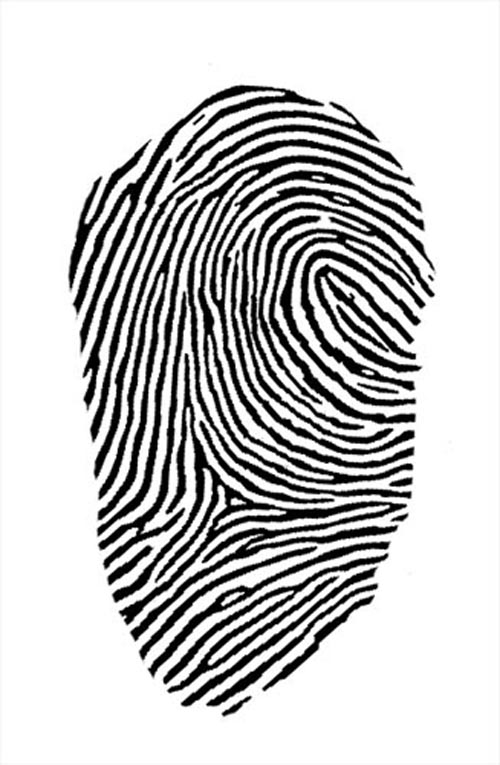
\includegraphics[height=0.7\textheight]{img/fingerabdruck.jpg}
  \end{figure}
\end{frame}

\begin{frame}
  \frametitle{Chaos Computer Club}
  \begin{figure}
    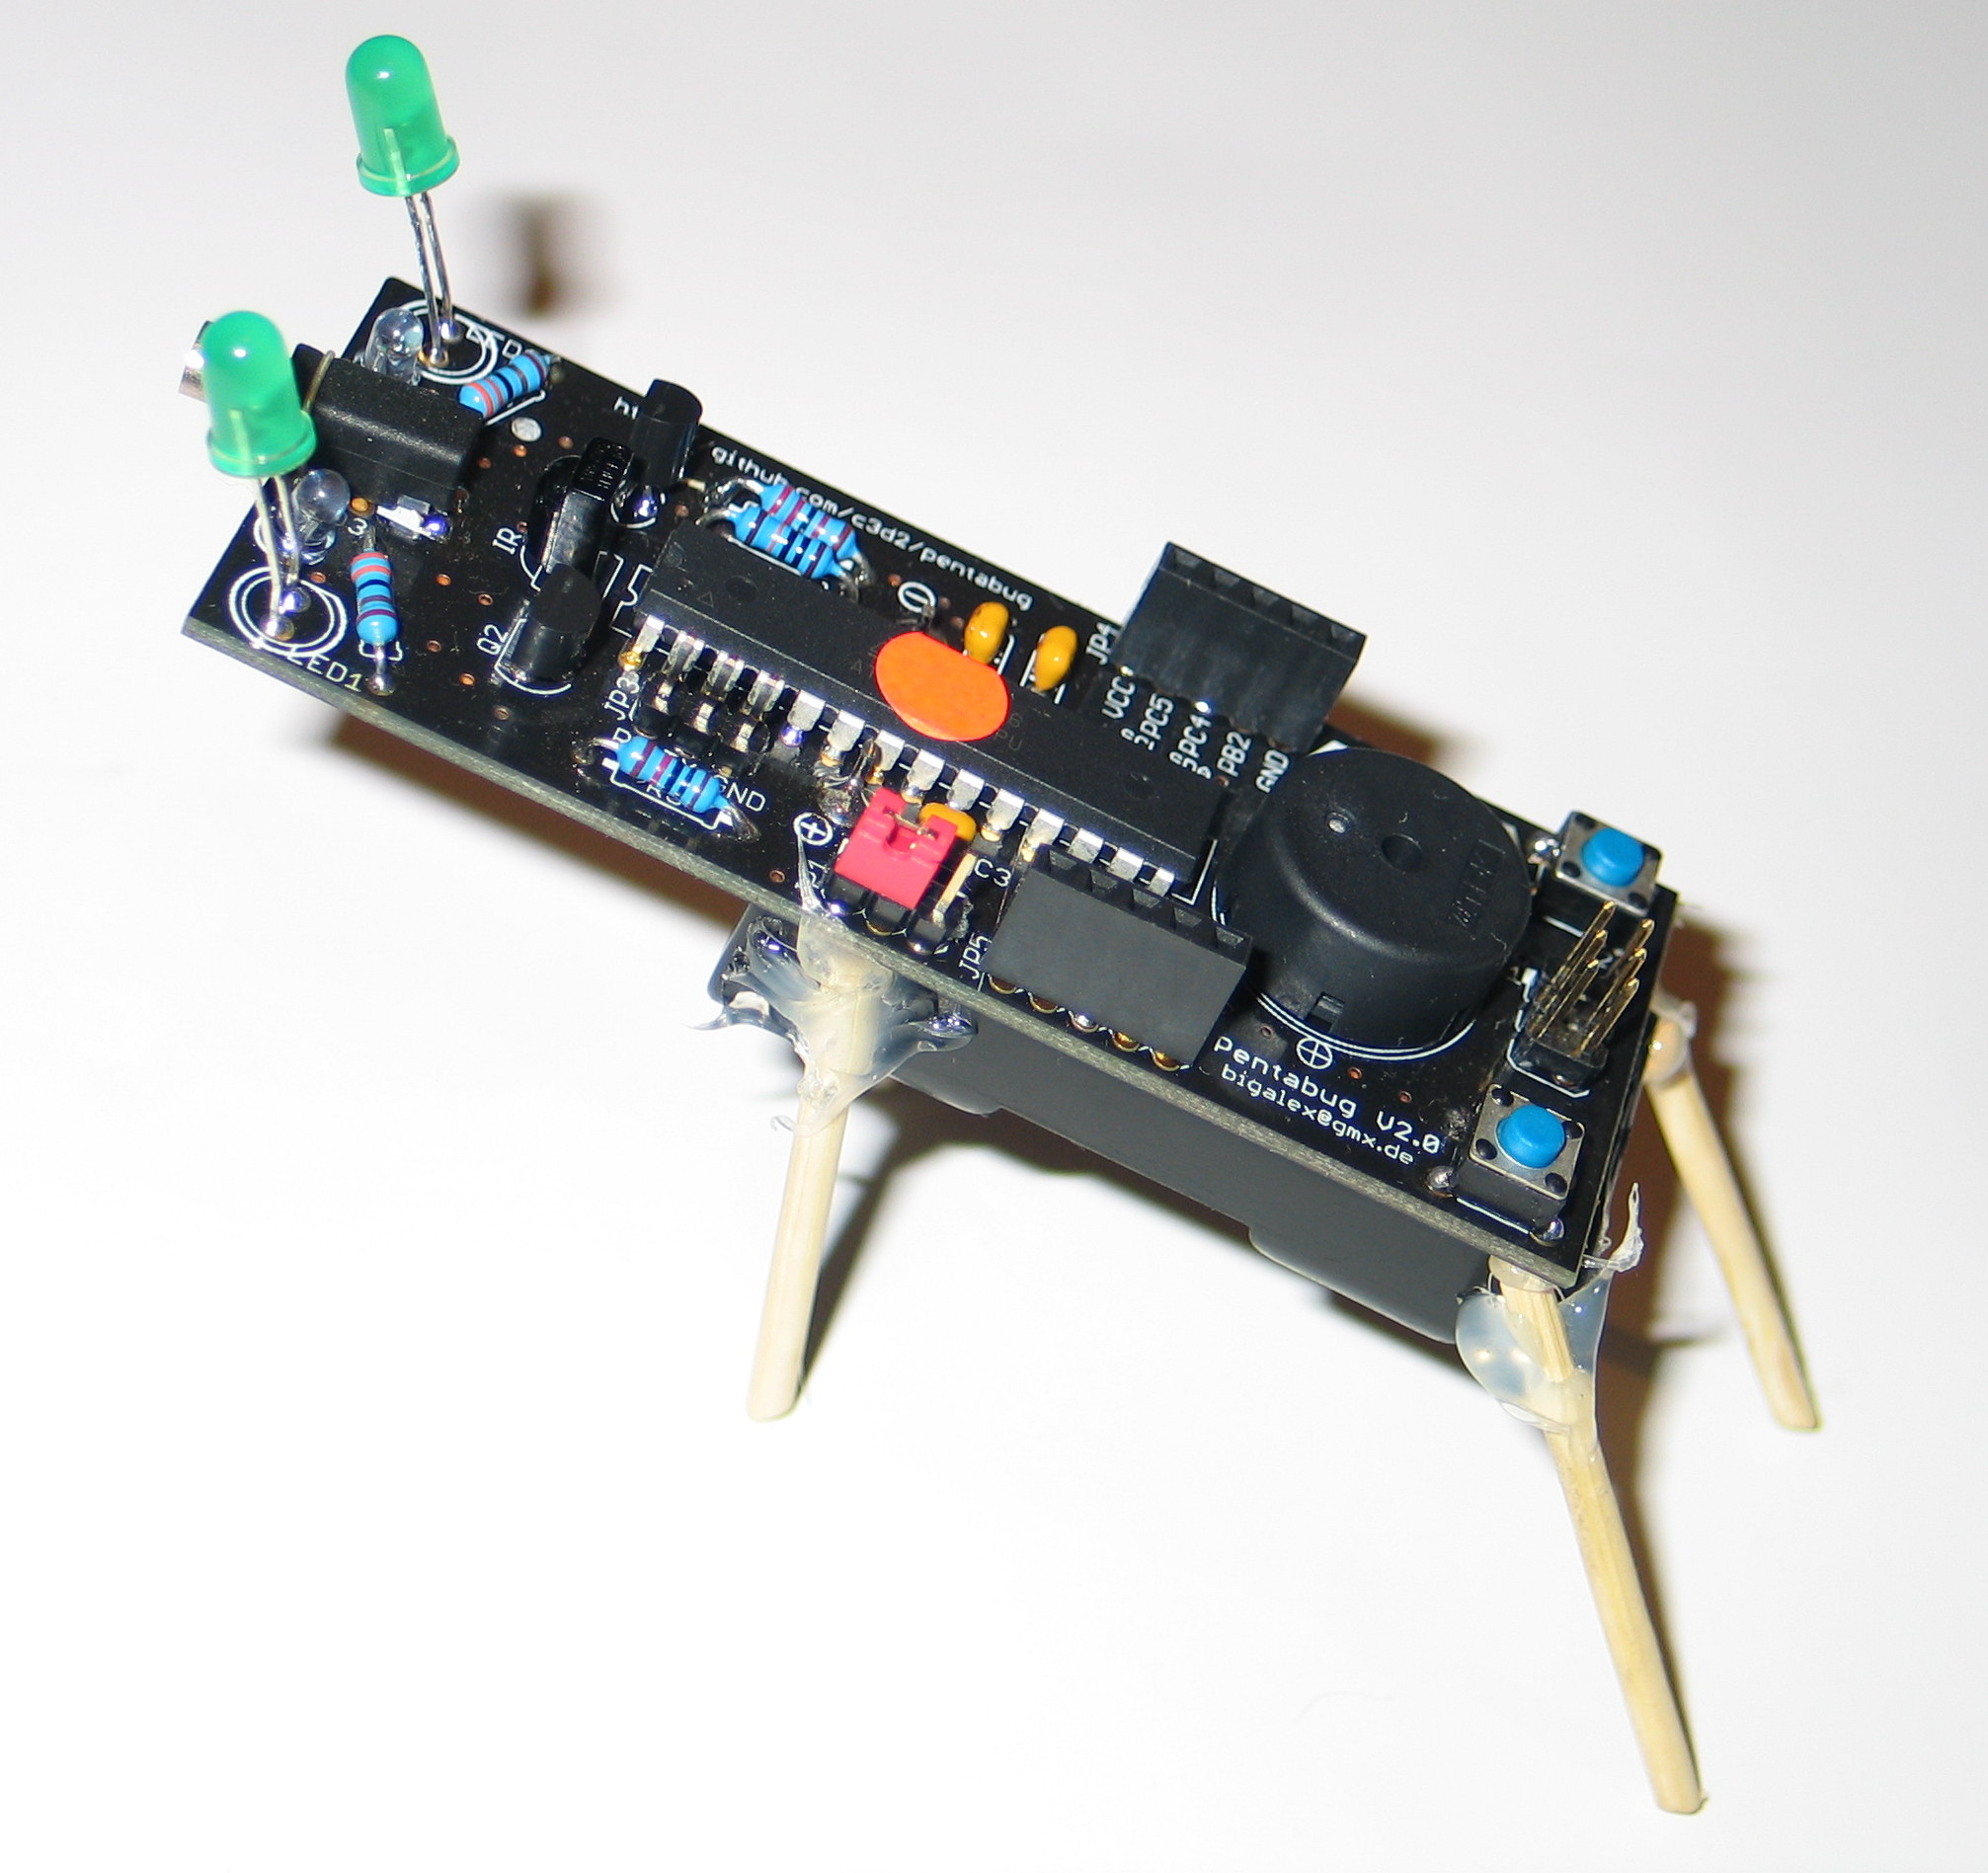
\includegraphics[height=0.7\textheight]{img/pentabug.jpg}
  \end{figure}
\end{frame}

\begin{frame}
    \frametitle{Chaos Computer Club}
    \begin{center}
  
\includegraphics[height=0.2\textheight]{img/chaosknoten.png}
    \end{center}
    \begin{itemize}
      \item<1-> Verein wurde 1981 gegr"undet (\url{https://ccc.de})
      \item<2-> Aktuell mehr als 6000 Mitglieder
      \item<3-> Betreibt u.a. "Offentlichkeitsarbeit und Politikberatung
      \item<4-> Lokale Erfahrungsaustauschkreise (Erfas) und Chaostreffs
      \item<5-> Chaos Communication Congress
    \end{itemize}
\end{frame}

\begin{frame}
  \frametitle{Chaos Computer Club Dresden}
  \begin{center}
    
\includegraphics[height=0.1\textheight]{img/c3d2_logo.png}
  \end{center}
  \begin{itemize}
    \item<1-> Chaos Computer Club Dresden (\url{https://c3d2.de})
    \item<2-> Datenspuren (\url{https://datenspuren.de})
    \item<3-> Radio und Podcasts (\url{https://c3d2.de/radio.html})
    \item<4-> Chaos macht Schule (\url{https://c3d2.de/schule.html})
  \end{itemize}
\end{frame}

\section{Übersicht}
\subsection{}

\begin{frame}
  \frametitle{Text- and Datamining}
  \begin{center}
    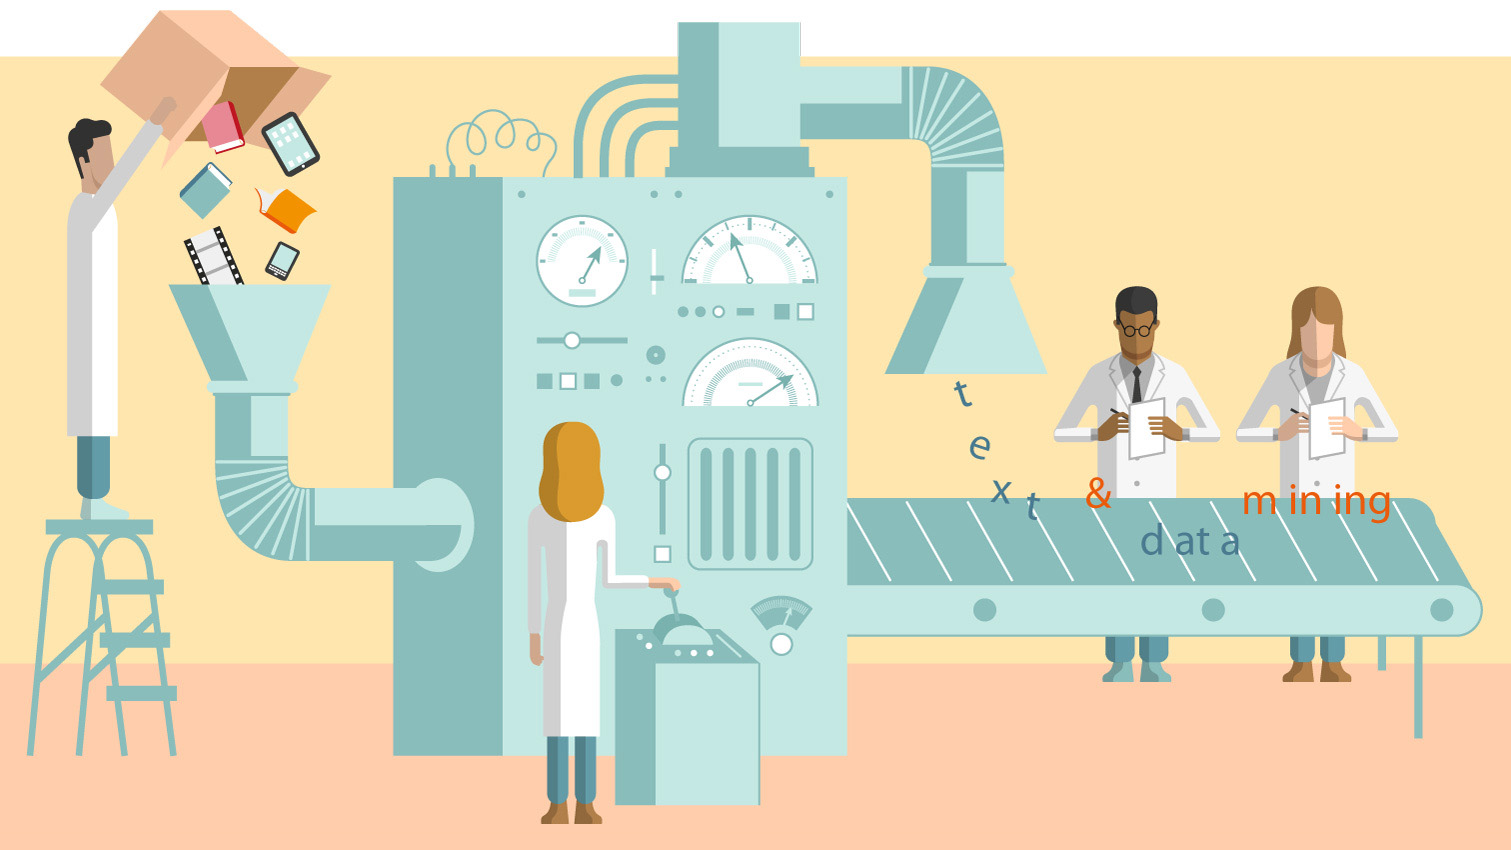
\includegraphics[width=0.9\textwidth]{img/text_data_mining.jpg} \\
    \tiny \cc{by} Maurizio Borghi - http://copyrightuser.org/topics/text-and-data-mining/
  \end{center}
\end{frame}

\begin{frame}
  \frametitle{Künstliche Intelligenz}
  \only<2> {
    \begin{columns}
      \begin{column}{0.5 \textwidth}
        \begin{center}
          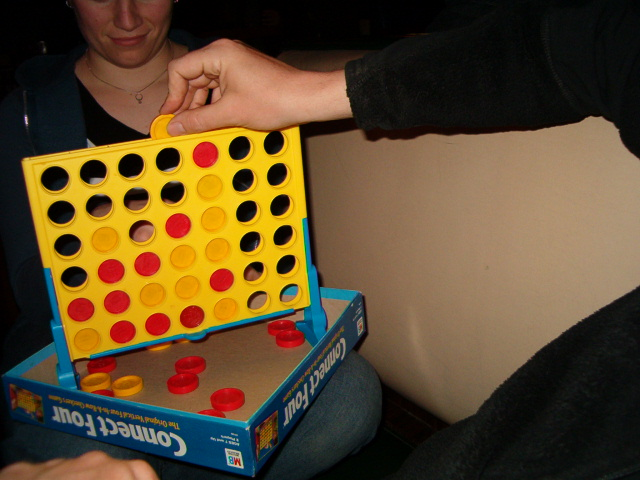
\includegraphics[width=0.8\textwidth]{img/connect_four.jpg} \\
          \tiny \cc{by} Jonathan Kellenberg \\ http://flickr.com/photos/72613214@N00
        \end{center}
      \end{column}
      \begin{column}{0.5 \textwidth}
        \begin{center}
          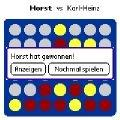
\includegraphics[width=0.4\textwidth]{img/4_gewinnt.jpg} \\
        \end{center}
      \end{column}
    \end{columns}
  }
  \only<3> {
    \begin{columns}
      \begin{column}{0.5 \textwidth}
        \begin{center}
          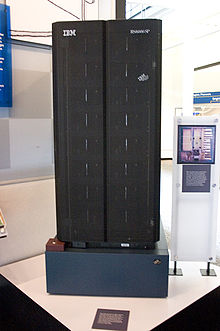
\includegraphics[width=0.6\textwidth]{img/deep_blue.jpg} \\
          \tiny \cc{by} James the photographer \\ http://flickr.com/photos/22453761@N00
        \end{center}
      \end{column}
      \begin{column}{0.5 \textwidth}
        \begin{center}
          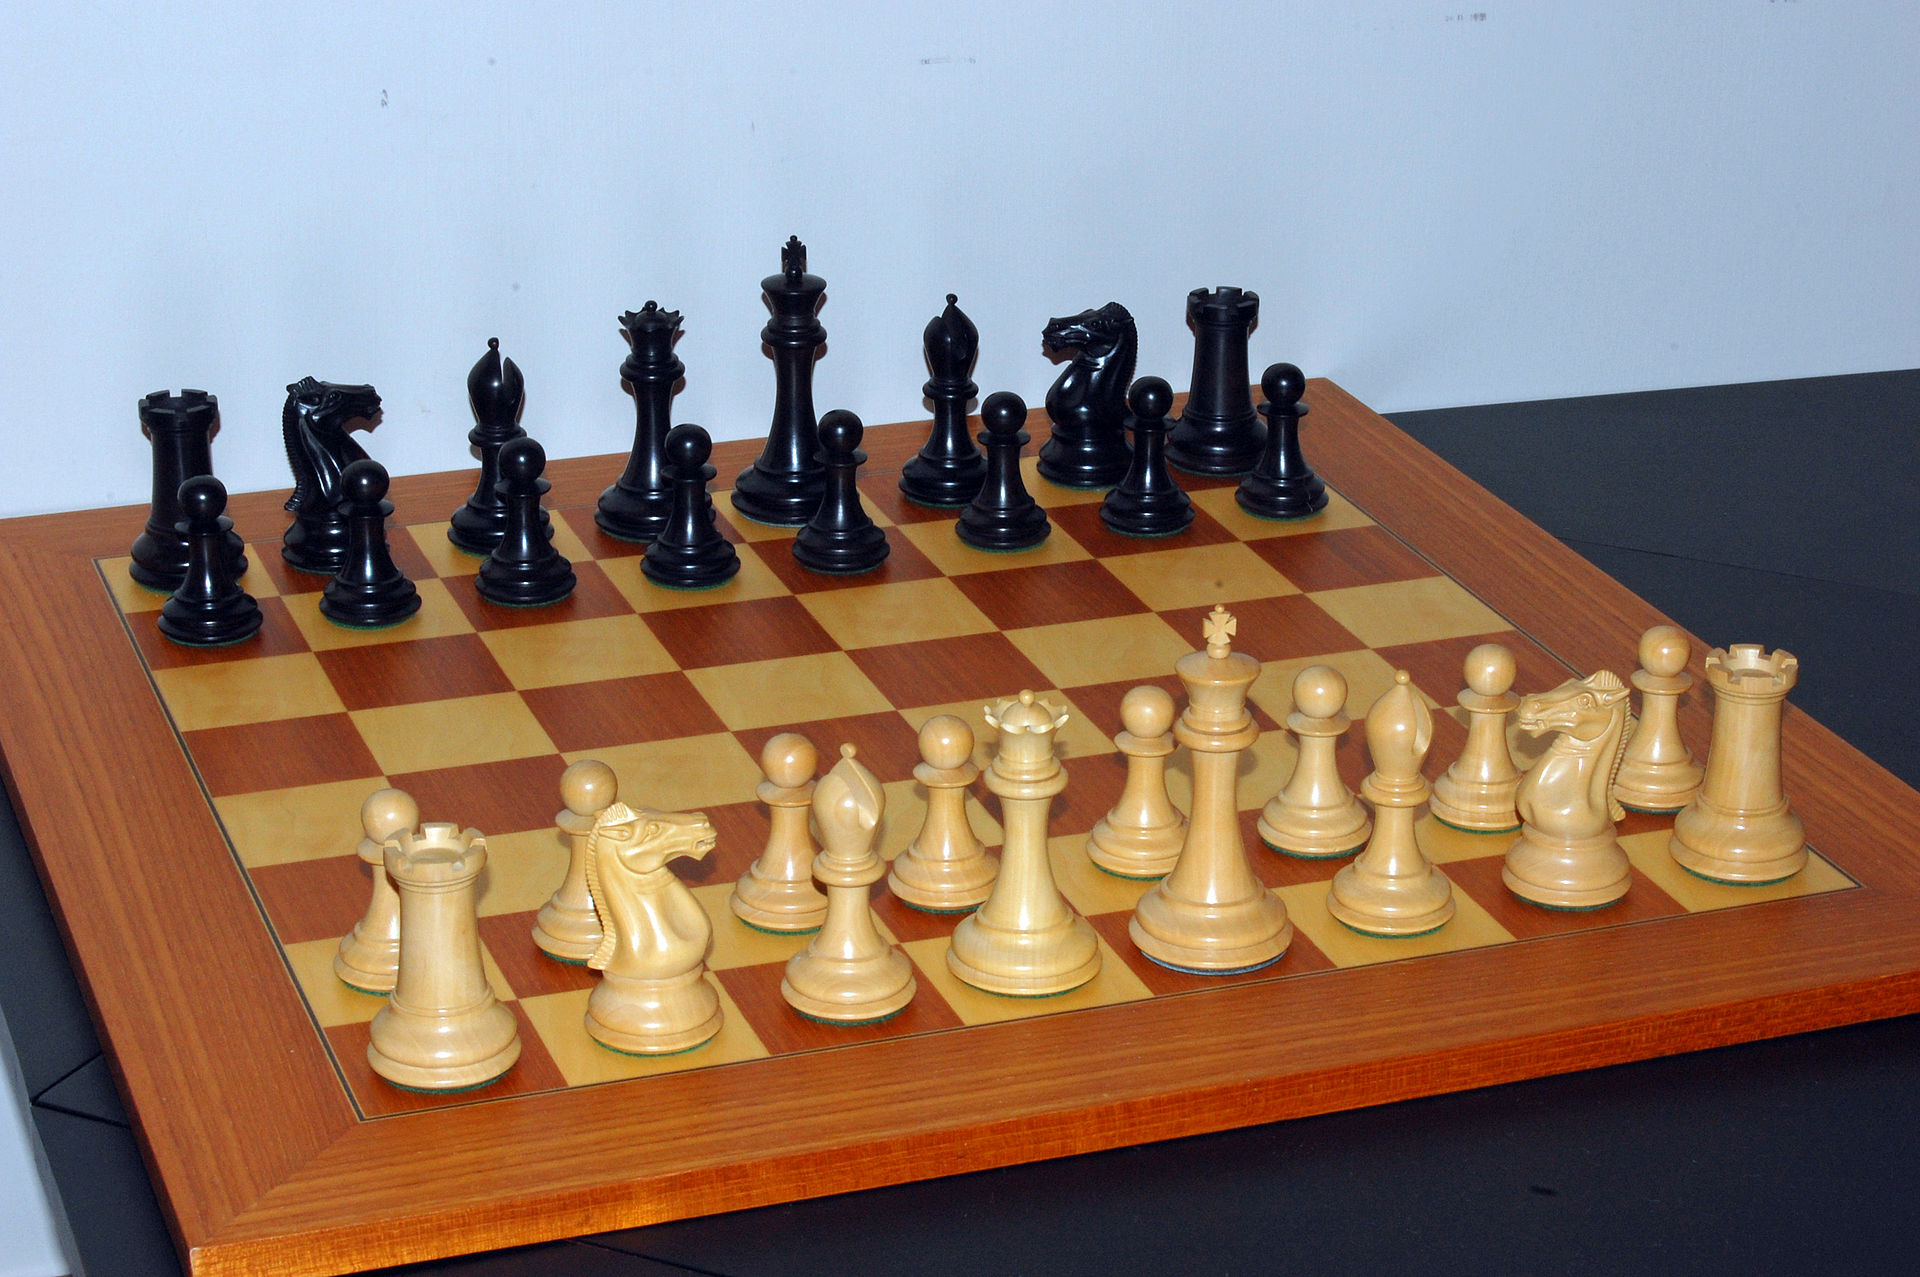
\includegraphics[width=0.8\textwidth]{img/chess.jpg} \\
          \tiny \cc{by-sa} Bubba73
        \end{center}
      \end{column}
    \end{columns}
  }
  \only<4> {
    \begin{center}
      
\includegraphics[width=0.4\textwidth]{img/alpha_go.png} \\

      \vspace{0.5cm}

      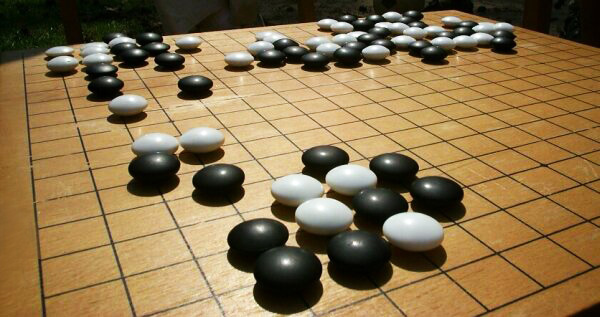
\includegraphics[width=0.6\textwidth]{img/go_board.jpg} \\
      \tiny \cc{by} Donarreiskoffer
    \end{center}
  }
\end{frame}

\section{Feste Regeln}
\subsection{}

\begin{frame}
  \frametitle{Gezielte Werbung}
  \begin{center}
    
\includegraphics[width=0.6\textwidth]{img/adwords.png} \\
  \end{center}
\end{frame}

\begin{frame}
  \frametitle{Social Bots}
  \begin{columns}
    \begin{column}{0.7 \textwidth}
      \begin{itemize}
        \item<2-> Spam der sozialen Netzwerke
        \item<3-> Überwachung von Schlagwörtern
        \item<4-> Trend-Setting
        \item<5-> basierend auf echten Profilen
      \end{itemize}
    \end{column}
    \begin{column}{0.3 \textwidth}
      \begin{center}
        
\includegraphics[width=\textwidth]{img/bot.png} \\
        \tiny \cc{by-sa} GNOME icon artists and Krzysztof Franek
      \end{center}
    \end{column}
  \end{columns}
\end{frame}

\begin{frame}
  \frametitle{Politik}
  \begin{center}
    \only<2> {
      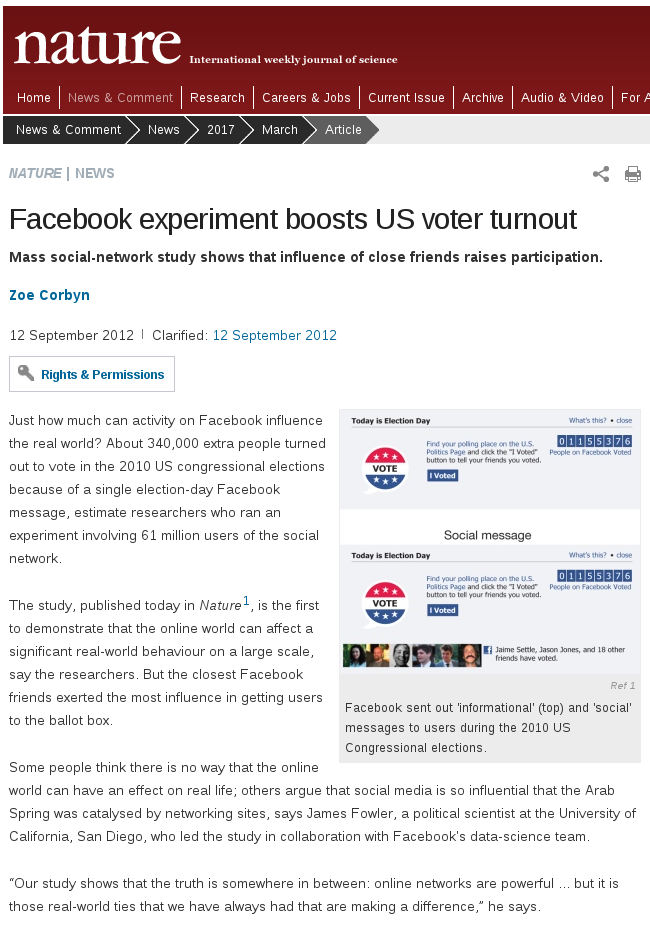
\includegraphics[height=0.7\textheight]{img/facebook_vote.png}
      % http://www.nature.com/news/facebook-experiment-boosts-us-voter-turnout-1.11401
      \\ \tiny www.nature.com
    }
    \only<3> {
      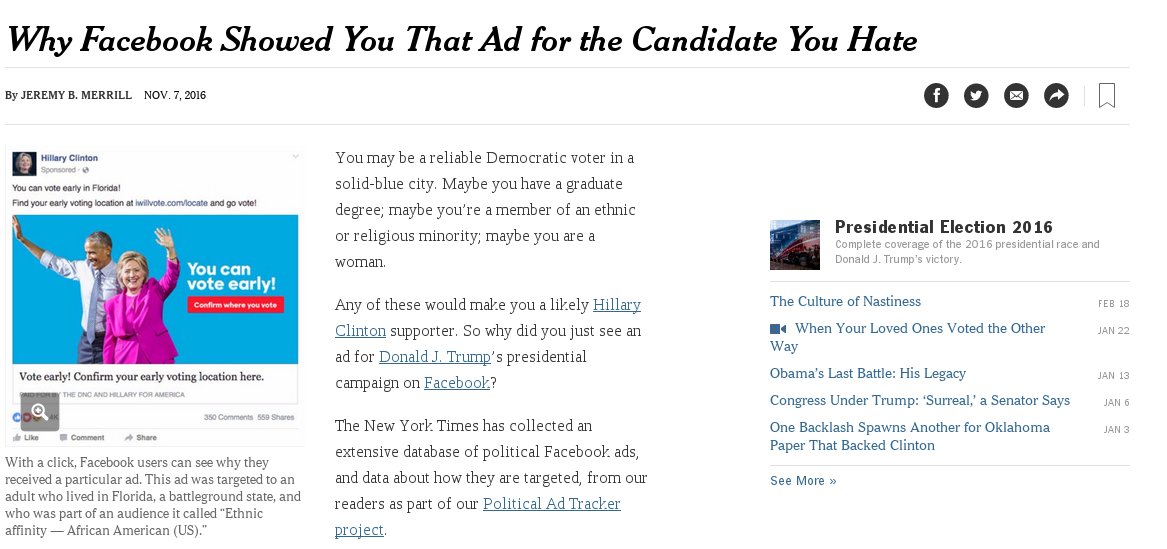
\includegraphics[height=0.5\textheight]{img/presidential.png}
      % https://www.nytimes.com/2016/11/08/us/politics/facebook-ads-campaign.html?_r=0
      \\ \tiny www.nytimes.com
    }
  \end{center}
\end{frame}

\section{Maschinelles Lernen}
\subsection{}

\begin{frame}
  \frametitle{Kaufverhalten}
  \pause
  \begin{center}
    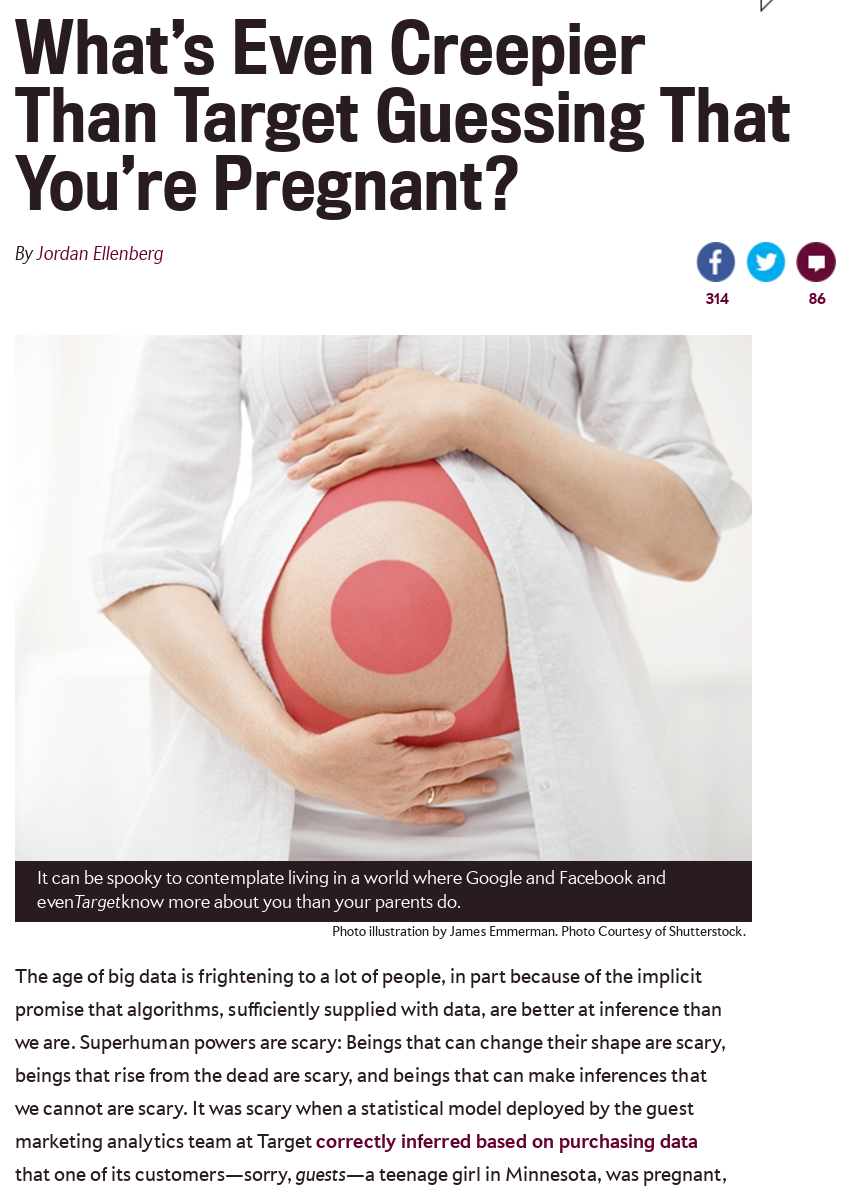
\includegraphics[width=0.4\textwidth]{img/pregnant.png} \\
    %\tiny http://www.slate.com/blogs/how_not_to_be_wrong/2014/06/09/big_data_what_s_even_creepier_than_target_guessing_that_you_re_pregnant.html
    \tiny http://www.slate.com/
  \end{center}
\end{frame}

\begin{frame}
  \frametitle{Beispiel}
  \only<1> {
    \begin{center}
      \begin{tabular}{l | c | c | c | c | c | c | c}
                & \rotatebox{90}{Brot} & \rotatebox{90}{Eier} & \rotatebox{90}{Milch} & \rotatebox{90}{Kuchen} & \rotatebox{90}{Ballons} & \rotatebox{90}{Pizza} & \rotatebox{90}{Käse} \\ \hline
        Becker  & x                     & x                   &                       & x                      &                         &                       & x                    \\ \hline
        Kaiser  & x                     &                     & x                     &                        &                         &                       & x                    \\ \hline
        Hoffmann  & x                     &                     & x                     &                        &                         & x                     &                      \\ \hline
        Meier   &                       & x                   &                       & x                      & x                       & x                     &                      \\ \hline
        Müller  &                       &                     & x                     & x                      & x                       &                       & x
      \end{tabular}
    \end{center}
  }

  \only<2> {
    \begin{center}
      \begin{tabular}{l | c | c | c | c | c | c | c}
                            & \rotatebox{90}{Brot} & \rotatebox{90}{Eier} & \rotatebox{90}{Milch} & \rotatebox{90}{Kuchen} & \rotatebox{90}{Ballons} & \rotatebox{90}{Pizza} & \rotatebox{90}{Käse} \\ \hline
        Becker              & x                     & x                   &                       & x                      &                         &                       & x                    \\ \hline
        Kaiser              & x                     &                     & x                     &                        &                         &                       & x                    \\ \hline
        Hoffmann              & x                     &                     & x                     &                        &                         & x                     &                      \\ \hline
        \color{red} Meier   &                       & x                   &                       & x                      & x                       & x                     &                      \\ \hline
        \color{red} Müller  &                       &                     & x                     & x                      & x                       &                       & x
      \end{tabular}
    \end{center}
  }

  \only<3> {
    \begin{center}
      \begin{tabular}{l | c | c | c | c | c | c | c}
                            & \rotatebox{90}{Brot} & \rotatebox{90}{Eier} & \rotatebox{90}{Milch} & \rotatebox{90}{Kuchen} & \rotatebox{90}{Ballons} & \rotatebox{90}{Pizza} & \rotatebox{90}{Käse} \\ \hline
        Becker              & x                     & x                   &                       & x                      &                         &                       & x                    \\ \hline
        Kaiser              & x                     &                     & x                     &                        &                         &                       & x                    \\ \hline
        Hoffmann              & x                     &                     & x                     &                        &                         & x                     &                      \\ \hline
        \color{red} Meier   &                       & x                   &                       & \color{red} x          & \color{red} x           & x                     &                      \\ \hline
        \color{red} Müller  &                       &                     & x                     & \color{red} x          & \color{red} x           &                       & x
      \end{tabular}
    \end{center}
  }

  \only<4> {
    \begin{center}
      \begin{tabular}{l | c | c | c | c | c | c | c}
                            & \rotatebox{90}{Brot} & \rotatebox{90}{Eier} & \rotatebox{90}{Milch} & \rotatebox{90}{Kuchen} & \rotatebox{90}{Ballons} & \rotatebox{90}{Pizza} & \rotatebox{90}{Käse} \\ \hline
        Becker              & x                     & x                   &                       & x                      &                         &                       & x                    \\ \hline
        Kaiser              & x                     &                     & x                     &                        &                         &                       & x                    \\ \hline
        Hoffmann              & x                     &                     & x                     &                        &                         & x                     &                      \\ \hline
        \color{red} Meier   &                       & x                   &                       & \color{red} x          & \color{red} x           & x                     &                      \\ \hline
        \color{red} Müller  &                       &                     & x                     & \color{red} x          & \color{red} x           &                       & x                    \\ \hline
        Sommer              & x                     & x                   &                       &                        &                         &                       & x                    \\ \hline
        Zimmer              &                       & x                   &                       & x                      & x                       & x                     &
      \end{tabular}
    \end{center}
  }

  \only<5> {
    \begin{center}
      \begin{tabular}{l | c | c | c | c | c | c | c}
                            & \rotatebox{90}{Brot} & \rotatebox{90}{Eier} & \rotatebox{90}{Milch} & \rotatebox{90}{Kuchen} & \rotatebox{90}{Ballons} & \rotatebox{90}{Pizza} & \rotatebox{90}{Käse} \\ \hline
        Becker              & x                     & x                   &                       & x                      &                         &                       & x                    \\ \hline
        Kaiser              & x                     &                     & x                     &                        &                         &                       & x                    \\ \hline
        Hoffmann              & x                     &                     & x                     &                        &                         & x                     &                      \\ \hline
        \color{red} Meier   &                       & x                   &                       & \color{red} x          & \color{red} x           & x                     &                      \\ \hline
        \color{red} Müller  &                       &                     & x                     & \color{red} x          & \color{red} x           &                       & x                    \\ \hline
        Sommer              & x                     & x                   &                       &                        &                         &                       & x                    \\ \hline
        \color{red} Zimmer  &                       & x                   &                       & \color{red} x          & \color{red} x           & x                     &
      \end{tabular}
    \end{center}
  }
\end{frame}

\begin{frame}
  \frametitle{Erkennung von Suchtverhalten}
  \only<1> {
    \begin{center}
      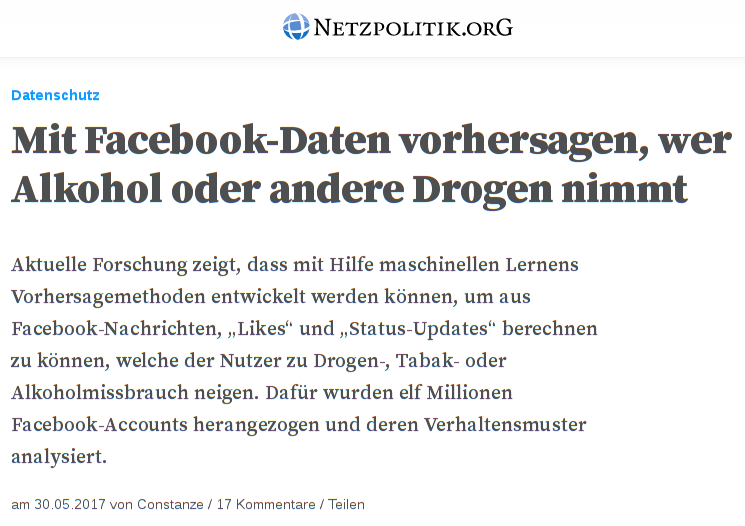
\includegraphics[width=0.7\textwidth]{img/facebook_drogen.png} \\
      \tiny https://netzpolitik.org/2017/mit-facebook-daten-vorhersagen-wer-alkohol-oder-drogen-nimmt/
    \end{center}
  }
  \only<2> {
    \begin{itemize}
      \item 86\% Genauigkeit Tabaknutzung
      \item 84\% Genauigkeit Drogenkonsum
      \item 81\% Genauigkeit Alkoholkonsum
      \item Identifizierung von Wörtern/Themen mit Korrelation
    \end{itemize}
  }
\end{frame}

\section{Neuronale Netze}
\subsection{}

\begin{frame}
  \frametitle{Neuronale Netze}
  \begin{center}
    \only<1> {
      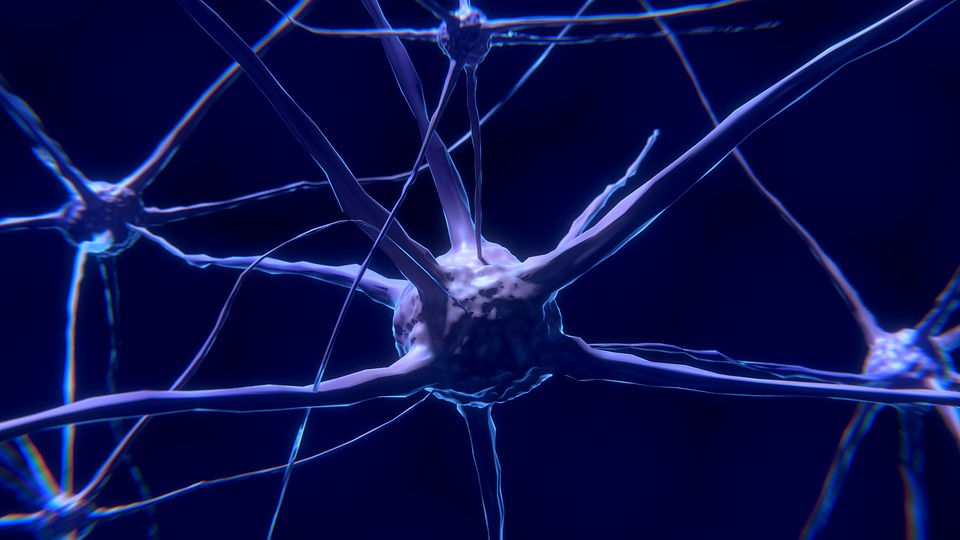
\includegraphics[width=0.7\textwidth]{img/neuron.jpg} \\
    }
    \only<2> {
      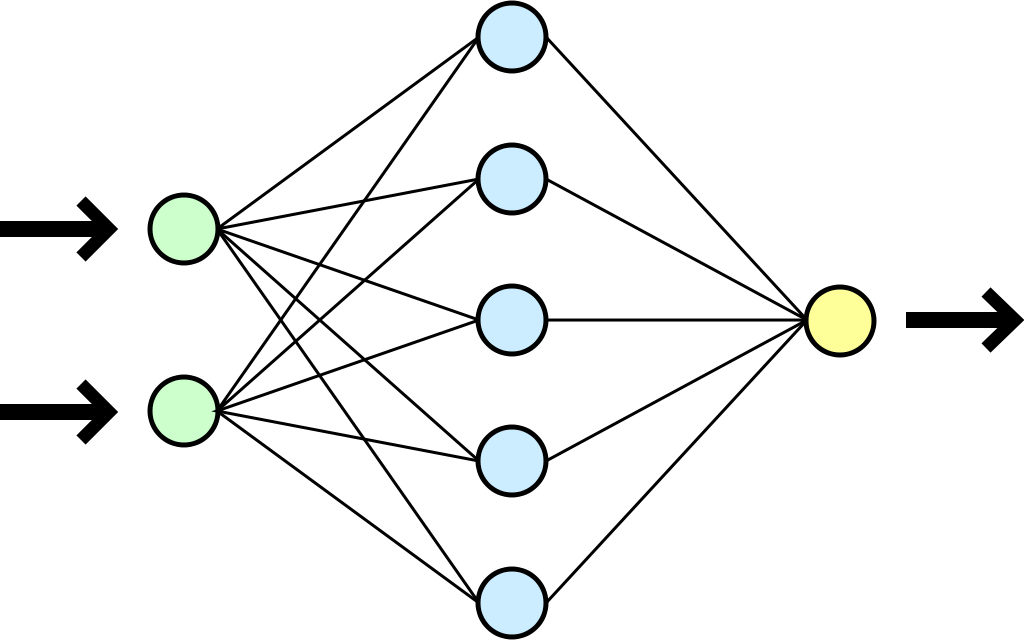
\includegraphics[width=0.7\textwidth]{img/network.png} \\
      \vspace{0.5cm}
      \tiny \cc{by} Dake, Mysid
    }
  \end{center}
\end{frame}

\begin{frame}
  \frametitle{Bilderkennung}
  \pause
  \begin{center}
    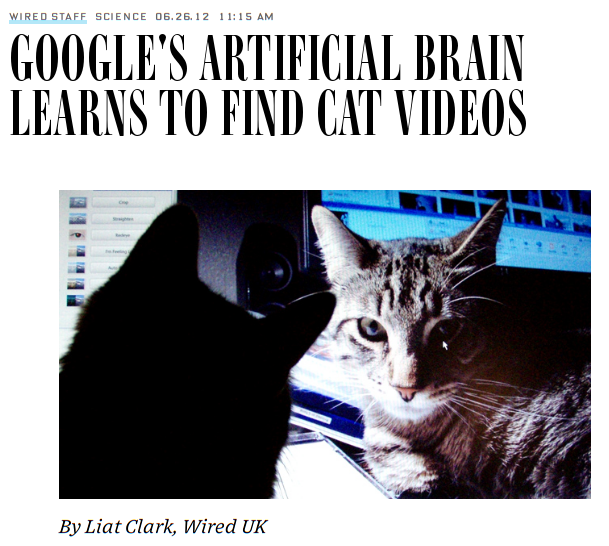
\includegraphics[width=0.6\textwidth]{img/cat_videos.png} \\
    \tiny https://www.wired.com/2012/06/google-x-neural-network/
  \end{center}
\end{frame}

\end{document}
